\documentclass{article}
\usepackage{graphicx}
\usepackage{subcaption}
 % Include the file specifying the document structure and custom commands
\title{UB304L: Assignment 2} % Title of the assignment

\author{Aditya Iyer\\ \texttt{adityaanant@iisc.ac.in}} % Author name and email address

\date{\today} % University, school and/or department name(s) and a date
\begin{document}

\maketitle % Print the title

\section*{Introduction} % Unnumbered section

Extracellular recordings from the ventral nerve cord of a cockroach were noted. Using this system, the effect of pharmacological intervention by nicotine and alcohol are identified. We show that nicotine increases firing rate, and alcohol reduces it.

Extracellular recordings from a decaptiated cockroach leg werer used to consider the effects of temperature on nerve firing. It is found that the firing rate and mean amplitude of spikes reduces as temperatures reduce.

Due to lack of computational power, I wasn't able to add peaks to all plots. An example is given on the first figure.


\section{Pharmacological Intervention} % Numbered section
Extracellcular recordings were taken from the ventral nerve cord, by hooking an electrode to it. A threshold of 0.038 units was set for discounting noise from analysis.

Communication at synapses is facilitated by chemical signals, called neurotransmitters. Acetylcholine is one such neurotransmitter. Neurons having Acetylcholine receptors are cholinergic neurons.

Nicotine affects these cholinergic neurons. It imitiates Acetylcholine and competively binds to ACh receptors, thereby activating firing.

Alcohol inhibits firing by affecting GABAergic neurons and activating potassium channels, increasing potassium ion efflux.

These explain the results of why firing increases drastically, as indicated in Figure 4.

The mean amplitudes do not vary much across treatments. This implies that the number of neurons firing remains the same.

\begin{figure}
  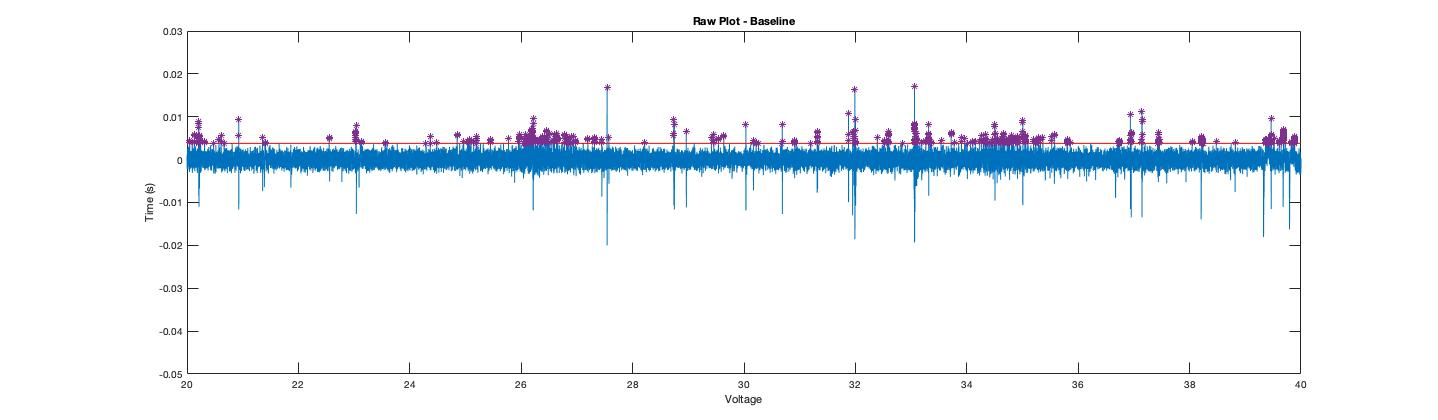
\includegraphics[width=\linewidth]{baseline.jpg}
  \caption{Raw Plot Showing Baseline Firing with threshold and labeled peaks}
  \label{fig: Raw Plot Showing Baseline Firing}
\end{figure}

\begin{figure}
  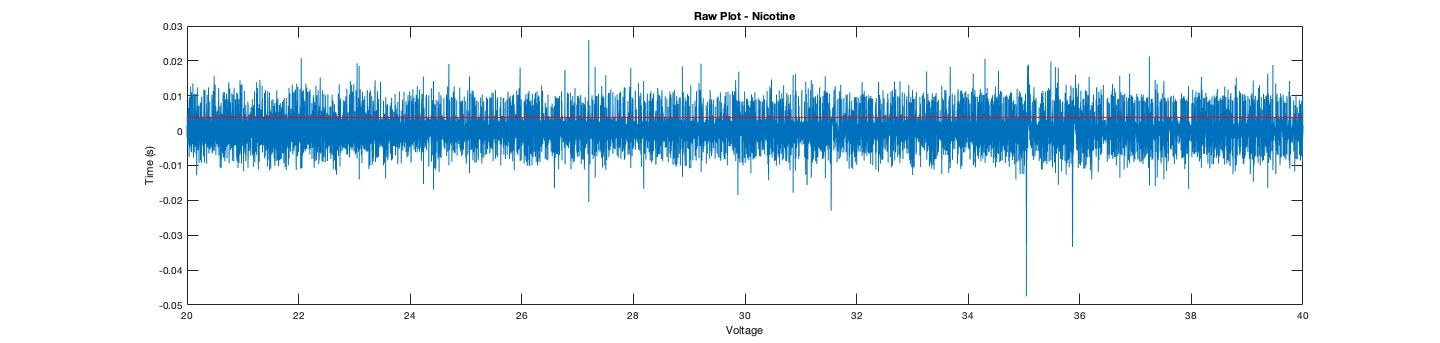
\includegraphics[width=\linewidth]{nicotine.jpg}
  \caption{Raw Plot of Ventral Nerve Cord Firing in Presence of Nicotine with threshold}
  \label{fig: Raw Plot of Ventral Nerve Cord Firing in Presence of Nicotine}
\end{figure}

\begin{figure}
  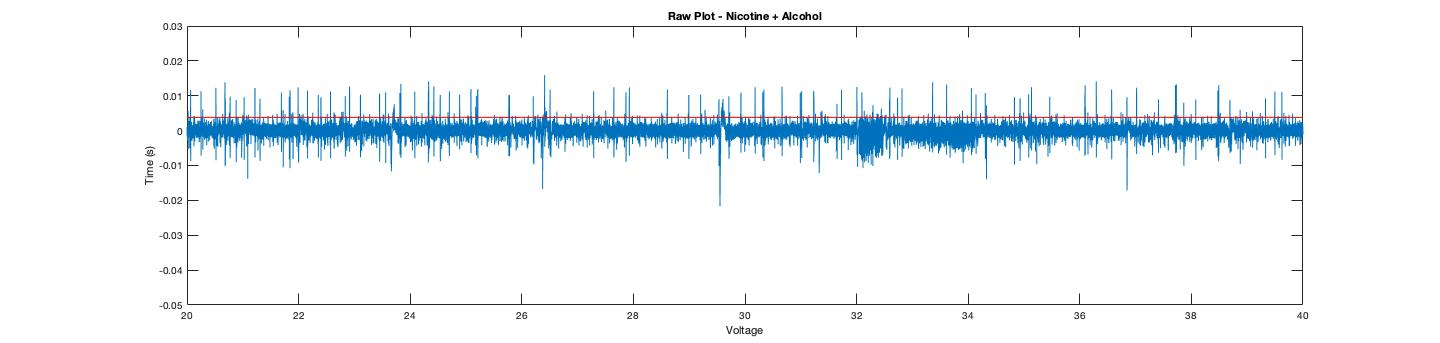
\includegraphics[width=\linewidth]{nical.jpg}
  \caption{Raw Plot of Ventral Nerve Cord Firing in Presence of Nicotine and Alcohol}
  \label{fig:  Raw Plot of Ventral Nerve Cord Firing in Presence of Nicotine and Alcohol}
\end{figure}


\begin{figure}[h!]
  \centering
  \begin{subfigure}{0.45\linewidth}
    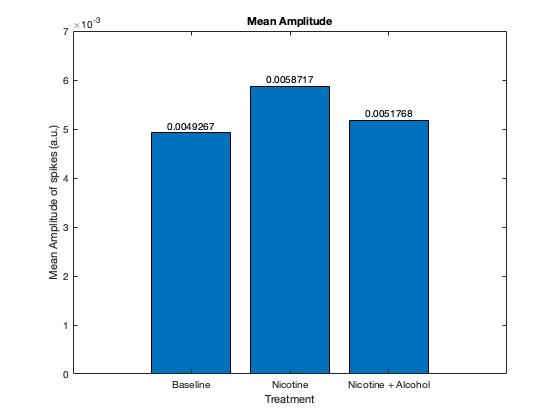
\includegraphics[width=\linewidth]{pharma-mean.jpg}
    \caption{fig: Mean Amplitude Across Treatments}
  \end{subfigure}
  \begin{subfigure}{0.45\linewidth}
    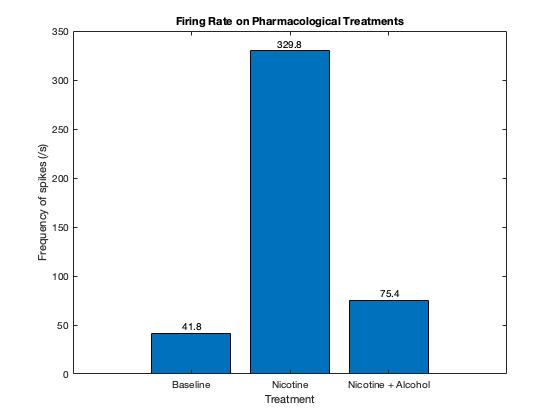
\includegraphics[width=\linewidth]{pharma-firing.jpg}
    \caption{Firing Rate Across Multiple Pharmacological Treatments}
  \end{subfigure}
  \caption{Bar Plots}
  \label{fig:pharma}
\end{figure}

\newpage

\section{Temperature Effects}

We recorded from a severed cockroach limb when at room temperature and after 5 minutes in ice (0C). The threshold for noise was set at 0.006 units.


When temperatures are low, the following are affected:
\begin{itemize}
	\item Resting Potential: Passive Transport of ions across the channel is affected by temperature, thereby changing the resting potential. This will reflect as changes in the amplitude of spikes.
	\item Ion Channel Transport: Active Transport of ions will also be affected by lower temperatures, (as dictated by statistical mechanics). This effect will present itself as change in firing rate
	\item Receptor Binding at Synapses will also be affected. Lower temperatures could imply lower binding rates and therefore, a lower firing rate.

All the above match our observation that firing rate and mean amplitude go down as temperature reduces, as shown in Figure 7.

\end{itemize}
\begin{figure}
	\centering
  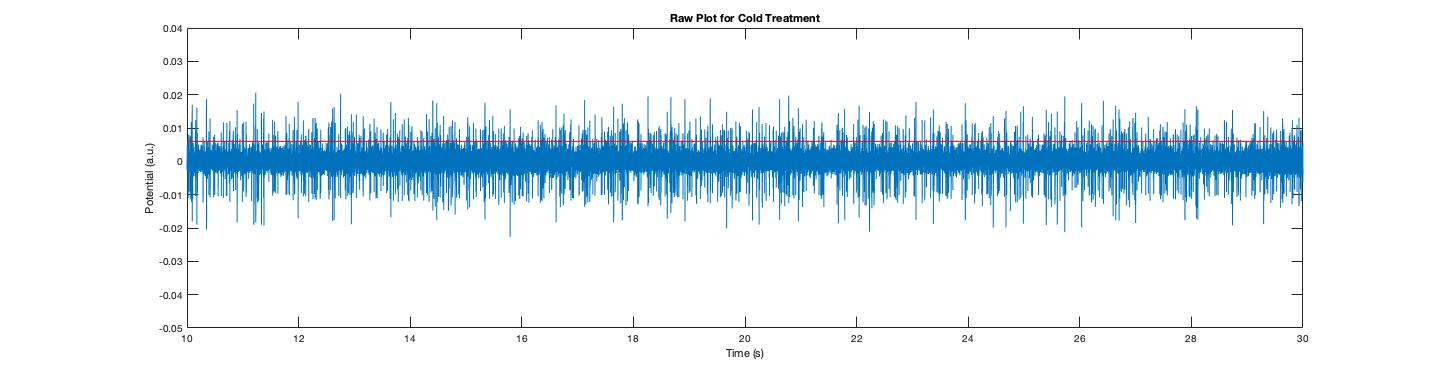
\includegraphics[width=\linewidth]{Cold_Raw.jpg}
  \caption{Raw Plot for Firing of Ventral Nerve Cord at Low Temperature}
  \label{fig:cold_raw}
\end{figure}

\begin{figure}
	\centering
  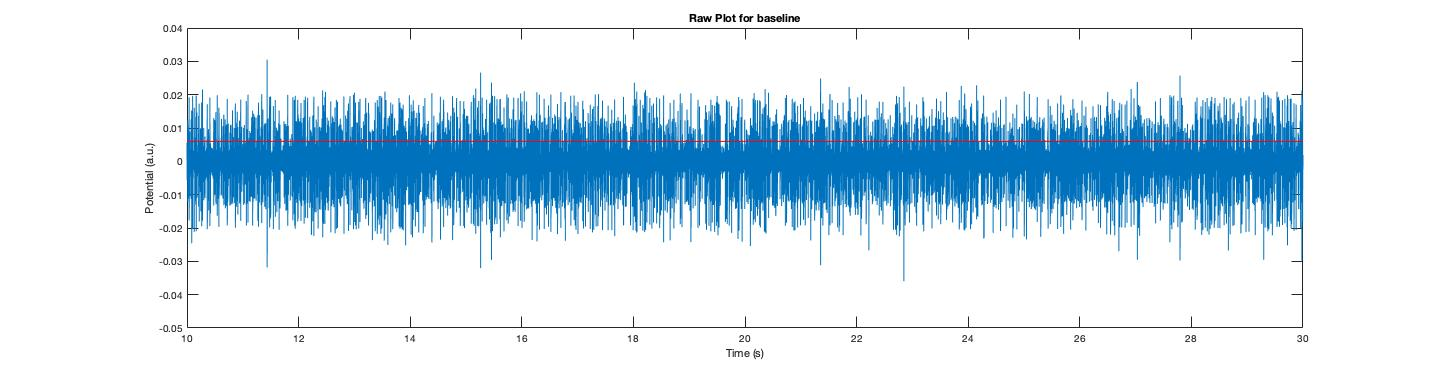
\includegraphics[width=\linewidth]{Temperature_Baseline.jpg}
  \caption{Raw Plot for Firing of Ventral Nerve Cord at Room Temperature}
  \label{fig:room_temp_raw}
\end{figure}


\begin{figure}[h!]
  \centering
  \begin{subfigure}{0.45\linewidth}
    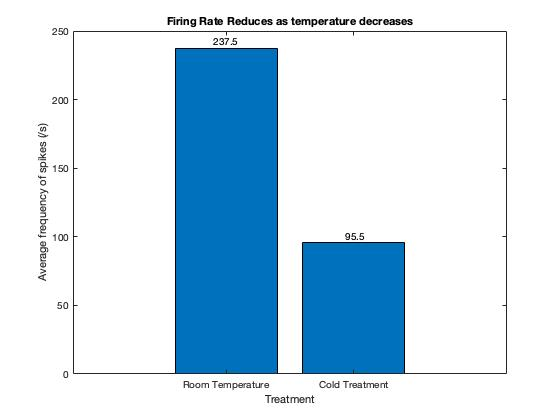
\includegraphics[width=\linewidth]{Firing_Temp.jpg}
    \caption{Bar Plot for Firing Rate across Temperatures}
  \end{subfigure}
  \begin{subfigure}{0.45\linewidth}
    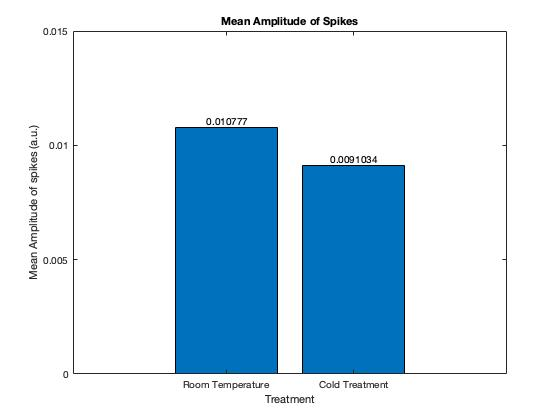
\includegraphics[width=\linewidth]{Mean_Temp.jpg}
    \caption{Bar Plot for Mean Amplitude of Spikes acorss Temperaturess}
  \end{subfigure}
  \caption{Bar Plots}
  \label{fig:pharma}
\end{figure}
%------------------------------------------------

%----------------------------------------------------------------------------------------

\newpage
\section{References}
\begin{enumerate}
	\item  C. Gotti, M. Zoli, Oncotarget; 2016, 7(50); 81977-81978; doi: 10.18.632/oncotarget13463
	\item Clark A, et al. Drug Alcohol Depend. 2004, ↓ Full text
Interactions between low concentrations of ethanol and nicotine on firing rate of ventral tegmental dopamine neurones,
\end{enumerate}

\vspace*{4\baselineskip}

\section{Extracellular Action Potential Shape}
\begin{figure}[h]
	\centering
  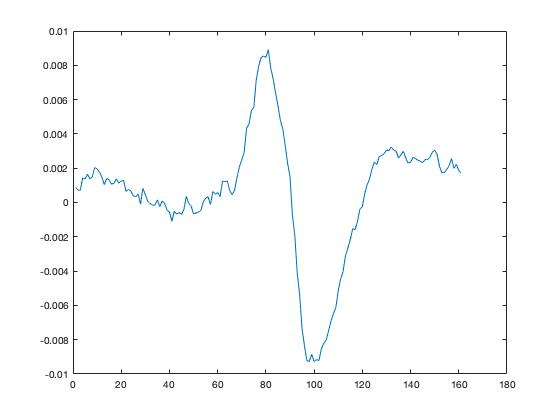
\includegraphics[width=\linewidth]{Action_Potential.jpg}
  \caption{Extracellular Action Potential}
  \label{fig:room_temp_raw}
\end{figure}

\end{document}
